
\documentclass[12pt]{article}
\usepackage[notext]{stix}
\usepackage{step}
\usepackage[T1]{fontenc}
\usepackage{amsmath}
\usepackage{amsfonts}
\usepackage[margin=2.5cm]{geometry}
\usepackage{titling}
\usepackage{listings}
\usepackage{titlesec}
\usepackage{parskip}
\usepackage[dvipsnames]{xcolor}
\usepackage{tikz}
\usepackage{hyperref}
\hypersetup{
    colorlinks=true,
    linkcolor=blue,
    filecolor=blue,      
    urlcolor=cyan,
    pdftitle={Overleaf Example},
    pdfpagemode=FullScreen,
    }

\usetikzlibrary{chains, scopes}
\tikzset{memory box/.style={
        draw, fill=#1, minimum width={width("Memory UVWXYZ")+6pt},
        align=center, minimum height=4ex,
        outer sep=0pt, % this will make the borders overlap nicely
    },
    memory size/.style={
        anchor=south east, font=\tiny, inner sep=1pt
    },
    memory address/.style={
         font=\tiny\ttfamily, inner ysep=1pt, inner xsep=3pt,
         anchor=#1 east,
    },
}

\lstset{ 
    language=C++, % choose the language of the code
    basicstyle=\fontfamily{pcr}\selectfont\footnotesize\color{red},
    keywordstyle=\color{red}\bfseries, % style for keywords
    numbers=none, % where to put the line-numbers
    numberstyle=\tiny, % the size of the fonts that are used for the line-numbers     
    backgroundcolor=\color{white},
    showspaces=false, % show spaces adding particular underscores
    showstringspaces=false, % underline spaces within strings
    showtabs=false, % show tabs within strings adding particular underscores
    frame=single, % adds a frame around the code
    tabsize=2, % sets default tabsize to 2 spaces
    rulesepcolor=\color{gray},
    rulecolor=\color{black},
    captionpos=b, % sets the caption-position to bottom
    breaklines=true, % sets automatic line breaking
    breakatwhitespace=false,
    commentstyle=\color{teal}, 
    emph={uint64_t},
    emphstyle=\color{blue}, 
}


\renewcommand\maketitlehooka{\null\mbox{}\vfill}
\renewcommand\maketitlehookd{\vfill\null}

\title{Operating Systems Notes}

\author{SubmergedDuck}
\date{\today}

\begin{document}
\begin{titlingpage}
\maketitle 
\end{titlingpage}

\newpage

\section{Page Tables: OSTEP {\hrule}}
\vspace{-1.5em}

    {\bf Paging.} {When memory is split into fixed-sized pieces. Inside one page,
    the offset tells "which byte within this page."} \par

    {\bf Page.} {A fixed size unit in a process's address space.} \par

\vspace{1em}
    {\bf Fig 1. 64-Byte Address Space in 128-Byte Physical Memory. TBC.}
\vspace{1em}
\begin{center}
    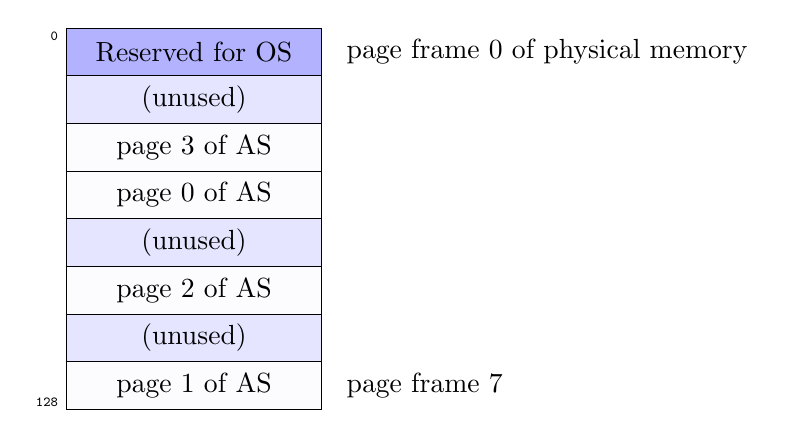
\begin{tikzpicture}[]
        \node [memory box=blue!1, anchor=south, label={[xshift=2mm]east:{page frame 7}}] (M0) {page 1 of AS};
        \node [memory box=blue!10, anchor=south] at (M0.north) (M1) {(unused)};
        \node [memory box=blue!1, anchor=south] at (M1.north) (M2) {page 2 of AS};
        \node [memory box=blue!10, anchor=south] at (M2.north) (M3) {(unused)};
        \node [memory box=blue!1, anchor=south] at (M3.north) (M4) {page 0 of AS};
        \node [memory box=blue!1, anchor=south] at (M4.north) (M5) {page 3 of AS};
        \node [memory box=blue!10, anchor=south] at (M5.north) (M6) {(unused)};        
        \node [memory box=blue!30, anchor=south, label={[xshift=2mm]east:{page frame 0 of physical memory}}] at (M6.north) (M7) {Reserved for OS};        

    %% Add the texts (just a couple, as example)
    %% add the size
        \node [memory size] at (M0.south east) {};
        \node [memory size] at (M1.south east) {};
    %% add the addresses. Probably you can use a macro to make this easier...
        \node [memory address=south] at (M0.south west) {128};
        \node [memory address=north] at (M0.north west) {};
        \node [memory address=south] at (M1.south west) {};
        \node [memory address=north] at (M1.north west) {};
        \node [memory address=north] at (M7.north west) {0};

    \end{tikzpicture}
\end{center}

{Notice how each page here is $128 \div 8 = 16$ bytes each. Notice also how the address space is can be scattered throughout physical memory.} \par

{\bf Free List.} {When an OS wishes to place a process's address space into physical memory, it keeps a free list of all free pages/page frames of the physical memory.}

{\bf Page Table.} {A data structure to record each where each virtual page of the address space is located in physical memory. Each process has their own page table.}

{\bf Address Translations.} {What the page table stores for each virtual page of the address space.}
    \begin{enumerate}
        \item[]{\bf Eg.} {Virtual Page 1 $\rightarrow$ Physical Frame 7}
        \item[] {\bf Eg.} {To translate a virtual address to a physical address, we keep the offset (the right-most bits), but change the VPN to PFN. Using Fig 1, since the virtual page number is 1 (01 in binary) and the physical frame number is 7 (111 in binary) then our physical adress would be 111 | [offset] while our virtual adress would be 01 | [offset]. }
    \end{enumerate}
\vspace{1em}

{\bf Offset.} {Indicates which byte a virtual address is on a virtual page.}

{\bf Page Table Entry (PTE).} {A 20-bit VPN implies there are $2^{20}$ address translations for each process. We need 4 bytes per PTE to hold the physical translation plus other stuff. So for a 32-bit address space there are $2^{20} * 4$ bytes = 4MB of memory needed for each page table.}

    \begin{enumerate}
        \item[] {\bf Note.} {So the number of page table entries is equal to the number of address translations. The number of address translations is related to how many bits a VPN has.}
    \end{enumerate}


    
\newpage
\section{Page Tables: Other {\hrule}}
\vspace{-1.5em}

    \noindent
    {\bf Offset Bits.} {How many bits to count all bytes in one page.} \par  

    {\bf Swap Offset.} {The index of the page-sized slot in the swap area (file/partion) where the whole page was written when it was swapped out.} \par

    \begin{enumerate}
        \item[]{\bf Eg.} {A 4KB page has $4096$ bytes. Since $4096 = 2^{12}$, the page offset uses 12 bits.} \par 
    \end{enumerate}
    \vspace{1em}

    \noindent{\bf Virtual Page Number (VPN).} {The index of a virtual page. These are the high bits of the virtual address.)} \par

    \begin{enumerate}
        \item[]{\bf Eg.} {Given a 32-bit virtual address and 4KB pages, there would be 20 bits left for the VPN (cause 4KB $= 2^{12}$ bytes). This implies that there are $2^{20}$ virtual pages if there are 20 VPN bits.} \par 
    \end{enumerate}
    \vspace{1em}

    \setlength{\parindent}{0pt} 
    {\bf Page Table Entry (PTE).} {One record in the page table that maps a virtual page to a physical frame and bits like valid/present, R/W/X permissions, dirty, accessed, etc. A single second-level page table holds 1024 PTEs.} \par
    
    \begin{enumerate}
        \item[]{\bf Note.} {Each page table entry has a Present(P) bit saying whether that virtual page is currently in RAM. P = 1 $\implies$ the mapping is valid and you can use the page table number. P = 0 $\implies$ otherwise (could be swapped out or not mapped.)}
    \end{enumerate}

\vspace{1em}
    {\bf Virtual Page.} {A fixed-size chunk (eg. 4KB) of a process's virtual address space.}
    \setlength{\parindent}{15pt} \par

    \begin{enumerate}
        \item[]{\bf Eg.} {With 4KB pages, every virtual address splits into a virtual page number (which page) + offset (which byte inside that page)} \par

        \item[]{\bf Eg 2.} {Let virtual address = 0x12345ABC. Then the offset would be 0xABC (low 12 bits) and the VPN would be 0x12345 given 4KB pages.} 
    \end{enumerate}

\vspace{1em}
\setlength{\parindent}{0pt} 

    {\bf Single-level Page Table.} {One big array indexed by the VPN; each slot is a PTE that says where that virtual page lives (which physical frame).} \par

    {\bf Second-level Page Table.} {Splits the VPN into PDI | PTI (10 | 10).} \par

    \begin{enumerate}
        \item[]{\bf Eg.} {There are $2^{20}$ page table entries, each entry is 4 bytes. The total size of the single page table would be $2^{20} \times 4$ bytes.} \par
    \end{enumerate}

\vspace{1em}

    {\bf Physical Frame.} {A 4KB chunck of RAM (or same size as page) where a virtual page's data lives when it's in memory.} 

    {\bf Physical Frame Number (PFN).} {The index of a 4KB physical frame in RAM. After page-table lookup, the PTE gives you the PFN plus status bits. Eg. Given 4KB pages, VA = [PFN | 12-bit Offset]}

    {\bf MiB.} {A mebibyte. 1 MiB $= 2^{20}$ bytes} 

    {\bf Page Directory Index (PDI).} {The first 10 bits of virtual address (VA). Selects which page table to use.} \par

    {\bf Page Table Index (PTI).} {The next 10 bits after PDI of VA. The Selects which PTE inside that page table.} \par
 




{\bf Bit Shifting} \par
\begin{lstlisting}[language=C, numbers=left, basicstyle=\ttfamily]
#define PAGE_SHIFT 12 // 4KB Pages
uint64_t physical_address = ((uint64_t)pfn << PAGE_SHIFT)|offset; 

\end{lstlisting}

{\bf Translation Lookaside Buffer (TLB).} {A tiny, very fast cache inside the MMU that stores recent virtual page number (VPN) to physical frame number translations (plus R/W/X/valid bits).} \par
\begin{enumerate}
        \item[]{\bf Hit.} {MMU find the mapping in the TLB so it can form the physical address without reading the page tables from memory. Memory Accesses Needed: 1.}
        \item[]{\bf Miss.} {MMU (or OS) must walk the page tables in memory to find the PTE, then it can access the data. Memory Accesses Needed: 3. } 
\end{enumerate}

{\bf Memory Management Unit (MMU).} {The hardware between the CPU and RAM that translates virtual addresses to physical using TLB and page tables. Also enforces R/W/X permissions and raises page faults if needed and updates accessed/dirty bits.} \par

{\bf Accessed Bit (A/R).} {Set by the hardware on any read or write to the page. OS uses it to tell which pages were recently used (eg. for replacement).}

{\bf Dirty Bit (D/modified).} {Set on any write. If a dirty page is evicted, it must be written back to disk; if clean it can be dropped.}

{\bf Dirty Page.} {A memory page that's been modified (written to) since it was loaded (its dirty bit is set.) If the OS evicts it, it must write it back to disk; a clean page (non-modified) can be dropped without writing.}

{\bf Page Fault.} {The PTE says the page isn't in RAM (invalid/not present), thus trapping to the OS to bring the page in.}


\newpage

\section{Lecture 15/16: Page Replacement Algorithms {\hrule}}
\vspace{-1.5em}

{\bf Policy Decisions for Virtual Memory Management} \vspace{-0.5em} \par {There are three types of policies we need to know.}
    \begin{enumerate}
        \item[]{\bf Fetch Policy.} {Policies that we use to decide when to fetch a page.}
        \item[]{\bf Placement Policy.} {Policies that we use to decide where to put the page.}
        \item[]{\bf Replacement Policy.} {Policies that we use to decide what page to evict to make room.} 
    \end{enumerate}

\vspace{1em}

{\bf Page Fetch Policies.} {There are two types of fetch policies.}
    \begin{enumerate}
        \item[1]{\bf Demand Paging.} {This is a when we only fetch a page when we actually reference it. }
        \item[2]{\bf Prepaging.} {This is when we fetch a page, we will fetch a little bit more, so when the next page fault comes around the data/content that we need for that page is already there. This is so we don't have the issue of "stalling twice."} 
    \end{enumerate}

\vspace{1em}

{\bf Page Placement Policies.} {Modern memory managemnent systems allow for any physical frames to hold any virtual page. This means that on most computers, any of the physical frames are equally good to hold any virtual page. This also means that memory management hardware can translate any virtual-to-physical mapping equally well. } 
    \begin{enumerate}
        \item[]{\bf Why would we prefer some virtual-to-physical over others?}
        \vspace{-0.5em}
        \begin{enumerate}
            \item [1]{\bf NUMA Multiprocessors.} {NUMA stands for non-uniform memory access. When we have a NUMA processor, some memory locations results in faster memory access than others. Eg. Any processor can access entire memory, but local memory is faster. }
            \item [2]{\bf Cache Performance.} {You want to pick physical frames that does not result in bad behaviour. Thus we have to choose physical pages to minimize cache conflicts.}
        \end{enumerate}
        \item[]{\bf Note.} {Placement policy will have a much smaller effect than fetch and replacement polciies if memory is limited.} 
    \end{enumerate}

\vspace{1em}
{\bf Page Replacement Policies.} {The main goal of a replacement algorithm is to reduce the {\bf fault rate} (how frequent a page fault occurs). We want to evict pages that will never be used again in the future, but this is hard to do cause we don't know the future, so we will pick to evict the page that won't be used for the longest period of time. }
    \begin{enumerate}
        \item[]{\bf How are replacement algorithms evaluated?}
        \vspace{-0.5em}
        \begin{enumerate}
            \item[] We take an input reference string (a list of addresses in the order that a program references them) and we count how many page faults occured, the lower the better.
        
        \end{enumerate}
        \item[]{\bf What does it mean to reference an address? }
        \vspace{-0.5em}
        \begin{enumerate}
            \item[] It means to use a variable or pointer to locate and access data in memory. 
        \end{enumerate}

    \end{enumerate}
Timestamp: 5:19

\section{Lecture 12: Paging and Address Translation {\hrule}} 

{\bf Compaction.} {The idea that we have something called a physical memory (RAM) and as we are assigning physical memory to processes, we can end up with holes inbetween allocations of memory. The purpose of compaction is to eliminate the small fragments in physical memory by relocating allocated space by consolidating them so we get 1 big free space in physical memory that we can use for other processes.}
    \begin{enumerate}
        \item[]{\bf Note.} {Compaction is not possible with the C memory allocation library. The C library uses something called dynamic partitioning. It's not possible because once malloc() returns an address to you, that address would be out of reach by the malloc library––this means that the malloc library cannot change the address that was returned and update it to something else.}
        \item[] {\bf Dynamic Partitioning.} {Opposite of fixed partitions. \href{run:https://www.youtube.com/watch?v=bQVARMOIwFg}{Video} }
    \end{enumerate}

{\bf Dynamic Relocation.} {Also known as execution-time binding of addresses. The purpose of this is to be able to do {\bf swapping} and {\bf compaction} at runtime. Dynamic relocation allows us to take a virtual address that the user process is using as its executing instructions and translating them to physical addresses.}
    \begin{enumerate}
        \item[]{\bf Note.} {This allows the OS to change the mapping between virtual and physical addresses whenever it wants––thus able to move data from one region of memory to another region of memory.}
        \item[] {\bf Regarding Compaction.} {We are able to change some of the virtual-to-physical address translations.}
        \item[] {\bf What's the minimum requirements to relocate fixed or dynamic partitions?} 
        \vspace{-0.5em}
        \begin{enumerate}
            \item[] All memory used by the process must be contiguous, which means no holes. 
        \end{enumerate}
    \end{enumerate}

{\bf Relocation Registers.} {What some CPU architectures, commonly, the older ones have. The basic idea is to translate physical addresses by doing an add opertation to the virtual address to get the corressponding physical address. }
    \begin{enumerate}
        \item[]{\bf Eg. Translating Addresses w/ Reloc. Reg.} {Let's say base address is 10, and we want to translate the virtual address 5. Then the physical address you get is 10+5 = 15. }
        \item[]{\bf Note.} {We also have to check that the base address is within the limits of a process's address space to protect overwriting memory that we lost to other processes. Sometimes the generated physical address does not even exist, eg. -200 physical address. }
        \item[]{\bf Base and Limit Reg.} {On CPUs that have a "base" and "limit" registers, the MMU uses these registers to store the base address and also a limit. These registers are updated whenever we do a kernel level context switch.}
        \begin{enumerate}
            \item[1]{\bf Base.} {When we restore registers for the next process, we load the {\bf base} register with the starting address of the physical address of that process.}
            \item[2]{\bf Limit.} {Limit register is set to the last logical address of that process. Purpose is to cap what range of physical addresses are valid.}
            \item[3]{\bf Load/Store.} {When we execute any memory reference instruction like load and store, the hardware will add the base address to the logical address (limit)} 
        \end{enumerate}
        \item[]{\bf Kernel-Level Context Switch.} {When we switch from one process to another.} 
        \item[]{\bf Logical Address.} {It's the same thing as a virtual address.} 
    \end{enumerate}
Timestamp: 8:22
\end{document}